\documentclass[a4paper,pdf]{article}
\usepackage{hyperref}
\usepackage{pdfpages} % http://mirror.unl.edu/ctan/macros/latex/contrib/pdfpages/pdfpages.pdf
\usepackage{booktabs} 
\usepackage[utf8]{inputenc}
\usepackage{sectsty}
\subsubsectionfont{\fontsize{12}{15}\selectfont}
\begin{document}




%%% DIT IS DE TITLE PAGE VOOR INFORMATIEKUNDE NIET VOOR AI OF INFORMATICA! 
%% GEBRUIK VOOR AI OF INFORMATICA JE EIGEN TITLEPAGE TEMPLATES\


\begin{center}

\vspace{2.5cm}

% [CHANGE] The title of your thesis. If your thesis has a subtitle, then this
% should appear right below the main title, in a smaller font.
\begin{Huge}
Het Manipuleren van de Tweede Kamerverkiezingen door Uitbuiting van de Voorkeursdrempel
%Ondervertegenwoordigde Bevolkingsgroepen Adequater Vertegenwoordigd in de Tweede Kamer
\end{Huge}

\vspace{1.5cm}

% [CHANGE] Your full name. In case of multiple names, you can include their
% initials as well, e.g. "Jan G.J. van der Wegge".
\emph{Auteur}\\
Micha\"{e}l Amir\\
% [CHANGE] Your student ID, as this has been assigned to you by the UvA
% administration.
10580247

\vspace{0.5cm}

% [DO NOT CHANGE]
Bachelor Scriptie\\
% [CHANGE] Whether your Bachelor thesis is 6 ECTS (regular) or 9 ECTS (Honours
% programme).
Credits: 12 EC

\vspace{0.5cm}

% [DO NOT CHANGE] The name of the educational programme.
Bachelor Opleiding Informatiekunde

\vspace{0.25cm}

% [DO NOT CHANGE] The addess of the educational programme.
Universiteit van Amsterdam\\
Faculteit der Natuurwetenschappen, Wiskunde en Informatica\\
Science Park 904\\
1098 XH Amsterdam

\vspace{1cm}
\begin{figure}[H]
\centering

	
\includegraphics[width=0.1\linewidth]{UVA.png}

\end{figure}


\vspace{1cm}

\emph{Begeleider \& Eerste Examinator}\\
% [CHANGE] The name of your supervisor. Include the titles of your supervisor,
% as well as the initials for *all* of his/her first names.
Dr. M. J. Marx

\vspace{0.25cm}

% [CHANGE] The address of the institute at which your supervisor is working.
% Be sure to include (1) institute (is appropriate), (2) faculty (if
% appropriate), (3) organisation name, (4) organisation address (2 lines).
ILPS, IvI\\
Faculteit der Natuurwetenschappen, Wiskunde en Informatica\\
Universiteit van Amsterdam\\
Science Park 904\\
1098 XH  Amsterdam

\vspace{1cm}

\emph{Tweede Examinator}\\
% [CHANGE] The name of your supervisor. Include the titles of your supervisor,
% as well as the initials for *all* of his/her first names.
Dr. J. A. C. Sandberg

\vspace{0.25cm}
IvI\\
Faculteit der Natuurwetenschappen, Wiskunde en Informatica\\
Universiteit van Amsterdam\\
Science Park 904\\
1098 XH  Amsterdam
\vspace{1cm}

% [CHANGE] The date at which you will finalize and submit your thesis.
20-06-2016
\thispagestyle{empty}

\end{center}



\pagebreak

\tableofcontents

\pagebreak

\begin{abstract}
% [CHANGE] 
\end{abstract}


\pagebreak


% Here you input all your sections in seperate files

\section{Introduction}
\label{sec:intro}
\begin{itemize}
\item Bevat je onderzoeksvraag (of vragen)
\item Plaatst je vraag in de bestaande literatuur.
\end{itemize}

Je onderzoeksvraag is leidend voor je hele scriptie. Alles wat je doet moet uiteindelijk terug te voeren zijn op 1 doel: het beantwoorden van die vraag. 

Typisch zal je het dan ook zo doen:

Mijn onderzoeksvraag is onderverdeeld in de volgende deelvragen:

\begin{description}
\item[RQ1] \ldots We   beantwoorden deze vraag  door het volgende te doen/ antwoord op de volgende vragen te vinden/ \ldots
\begin{enumerate}
\item Vragen op dit niveau kan je echt beantwoorden, en dat doe je in je Evaluatie sectie~\ref{sec:eva}.
\end{enumerate}
\item[RQ2] \ldots
\item[RQ3] \ldots
\end{description}

Je Evaluatie sectie~\ref{sec:eva} bevat evenveel subsecties als je deelvragen hebt. En in elke sectie beantwoord je dan die deelvraag met behulp van de vragen op het onderste niveau.

In je conclusies kan je dan je hoofdvraag gaan beantwoorden op basis van al het eerder vergaarde bewijs.


\paragraph{Overview of thesis}
Hier geef je even kort weer wat in elke sectie staat.
\section{Gerelateerd Werk}
\label{sec:rel}

Deze sectie bestaat uit een aantal "blokken", waarin je per blok de relevante literatuur beschrijft. 

Neem alleen literatuur op die van belang is voor jouw onderzoeksvraag en deelvragen.

Typisch heb je 1 blok voor je hoofdvraag en per deelvraag \textbf{RQi} een blok. 


\subsection{RQ1}

\subsection{RQ2}
\section{Data}
\label{sec:meth}


\subsection{Description of the data}
Data verzameling en beschrijving van de data jajaja

Hoe is de data verzameld, en hoe heb jij die data verkregen?


Wat staat er in de data? Niet alleen maar een technisch verhaal, maar ook inhoudelijk. DE lezer moet een goed idee krijgen over de technische inhoud en wat het betekent.

\pagebreak
\subsection{Wat plotjes en tabelletjes}

Zie het IPython Notebook \url{PandasAndLatex.ipynb} voor de code om vanuit pandas een poltje op te slaan en een dataframe als tabel op te slaan. Het werkt ideaal! 

De interrupties van Wilders staan beschreven in Figure~\ref{fig:wilders} en Tabel~~\ref{tab:Wilders}.


\begin{figure}
\begin{center}
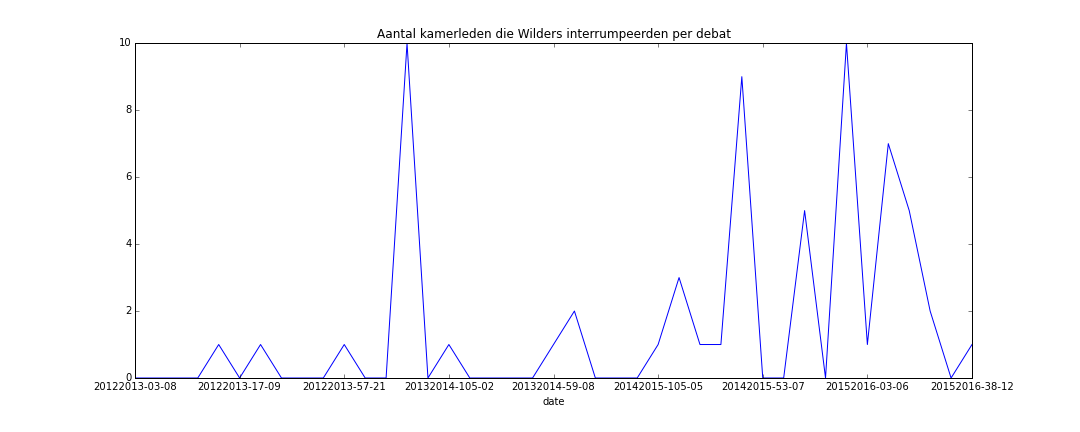
\includegraphics[width=\linewidth]{WildersPlot.png}
\caption{\label{fig:wilders} Aantal interrupties van Wilders in de Tweede Kamer door de tijd (periode 2012-2016).}
\end{center}
\end{figure}


\pagebreak

\begin{table}[h]
\begin{footnotesize}
\begin{tabular}{lrl}
\toprule
{} &  indegree &                               interruptie\_volgorde \\
date            &           &                                                    \\
\midrule
20122013-03-08  &         0 &                                                    \\
20122013-07-16  &         0 &                                                    \\
20122013-100-03 &         0 &                                                    \\
20122013-100-06 &         0 &                                                    \\
20122013-17-06  &         1 &                         Pechtold-Pechtold-Pechtold \\
20122013-17-09  &         0 &                                                    \\
20122013-21-04  &         1 &                         Pechtold-Pechtold-Pechtold \\
20122013-22-08  &         0 &                                                    \\
20122013-32-06  &         0 &                                                    \\
20122013-48-23  &         0 &                                                    \\
20122013-57-21  &         1 &  Pechtold-Pechtold-Pechtold-Pechtold-Pechtold-P... \\
20122013-76-03  &         0 &                                                    \\
20122013-76-06  &         0 &                                                    \\
20132014-05-02  &        10 &  Roemer-Roemer-Van Haersma Buma-Van Haersma Bum... \\
20132014-06-04  &         0 &                                                    \\
20132014-105-02 &         1 &  Pechtold-Pechtold-Pechtold-Pechtold-Pechtold-P... \\
20132014-105-06 &         0 &                                                    \\
20132014-14-03  &         0 &                                                    \\
20132014-14-06  &         0 &                                                    \\
20132014-52-18  &         0 &                                                    \\
20132014-59-08  &         1 &                               Klaver-Klaver-Klaver \\
20142015-02-08  &         2 &  Pechtold-Pechtold-Pechtold-Pechtold-Pechtold-P... \\
20142015-03-06  &         0 &                                                    \\
20142015-09-09  &         0 &                                                    \\
20142015-100-05 &         0 &                                                    \\
20142015-105-05 &         1 &                                  Pechtold-Pechtold \\
20142015-111-04 &         3 &  Pechtold-Pechtold-Pechtold-Pechtold-Pechtold-P... \\
20142015-111-07 &         1 &                                  Pechtold-Pechtold \\
20142015-39-71  &         1 &                                  Pechtold-Pechtold \\
20142015-41-07  &         9 &  Samsom-Samsom-Pechtold-Pechtold-Pechtold-Kuzu-... \\
20142015-53-07  &         0 &                                                    \\
20142015-61-23  &         0 &                                                    \\
20142015-79-07  &         5 &  Klaver-Klaver-Klaver-Gesthuizen-Gesthuizen-Ges... \\
20142015-95-06  &         0 &                                                    \\
20152016-02-07  &        10 &  Pechtold-Pechtold-Pechtold-Pechtold-Slob-Slob-... \\
20152016-03-06  &         1 &       Pechtold-Pechtold-Pechtold-Pechtold-Pechtold \\
20152016-14-02  &         7 &  Klaver-Klaver-Roemer-Roemer-Roemer-Roemer-Sams... \\
20152016-14-05  &         5 &  Van Haersma Buma-Van Haersma Buma-Van Haersma ... \\
20152016-27-03  &         2 &  Segers-Segers-Segers-Segers-Kuzu-Kuzu-Kuzu-Kuz... \\
20152016-38-10  &         0 &                                                    \\
20152016-38-12  &         1 &                                        Klein-Klein \\
\bottomrule
\end{tabular}

\end{footnotesize}
\caption{\label{tab:Wilders} Door wie werd Wilders onderbroken en hoe vaak per debat.}
\end{table}


\pagebreak
\subsection{Methods}
Hoe je je vraag gaat beantwoorden.


Dit is de langste sectie van je scriptie. 

Als iets erg technisch wordt kan je een deel naar de Appendix verplaatsen. 

Probeer er een lopend verhaal van te maken.

Het is heel handig dit ook weer op te delen nav je deelvragen:

\subsubsection{RQ1}

\subsubsection{RQ2}
\section{Theoretisch Maximum}
\label{sec:eva}

Met een subsectie voor elke deelvraag.

In hoeverre is je vraag beantwoord?

Een mooie graphic/visualisatie is hier heel gewenst.

Hou het kort maar krachtig.

\newpage
\subsection{Deelvraag 1: Wat is het theoretisch maxmimum aantal kandidaten dat per specifieke bevolkingsgroep gekozen kan worden in de Tweede Kamer?}

Om het theoretisch maximum te gaan berekenen zullen we als eerst kijken naar de verschillende specifieke bevolkingsgroepen zoals we deze hebben bepaald in de Methodologie sectie(of in de introductie. De specifieke bevolkingsgroepen moeten in ieder geval nog nader bepaald worden).

\subsubsection{Bevolkingsgroep: Vrouwen.}

Betreffende de bevolkingsgroep vrouwen in Nederland worden hieronder verschillende strategi\"{e}n uiteengezet om zodoende te achterhalen met welke strategie in theorie de meeste vrouwelijke kandidaten in de Tweede Kamer gekozen kunnen worden wanneer alle stemgerechtigde vrouwelijke kiezers in Nederland zich committeren aan de strategie.

\paragraph{Het berekenen van het totaal aantal stemmen en het totaal aantal stemmen door vrouwelijke kiezers per partij.}

Voor het opzetten van de strategi\"{e}n en het, voor elke strategie, kunnen toewijzen van de stemmen van vrouwelijke kiezers aan de vrouwelijke kandidaten van de partijen moeten we eerst weten hoeveel stemmen de partijen volgens de peiling zal gaan ontvangen. Dit doen we door de verwachte opkomst te delen door het aandeel zetels(in een percentage) dat een partij volgens de peiling zal ontvangen. Ter illustratie het volgende voorbeeld: In de peiling van 11 september 2012 werd er een opkomst van 73\% van alle stemgerechtigden verwacht . Er waren in 2012 een totaal aantal van 12.689.810 stemgerechtigden. Dat betekent dat 73\% van alle stemgerechtigden uitkomt op (0,73*12.689.810 = ) 9.263.561 verwachtte stemmen. Het aantal stemmen die een partij zou gaan ontvangen is dus het aandeel van het aantal zetels in de Tweede Kamer dat een partij zou gaan ontvangen volgens de peiling. Ter illustratie het volgende voorbeeld: de PVDA  zou, volgens de peiling,  36 zetels ontvangen. Dat komt neer op een percentage van (36/150 zetels = ) 24\% van alle zetels. Het aantal stemmen dat de PVDA daarmee zou gaan ontvangen is dan het aantal van (0,24*9.263.561 = ) 2.223.254 stemmen. Het percentage stemmen van de PVDA, dat volgens de peiling, van vrouwelijke kiezers zal komen is 48\%. Daarmee zal de PVDA het totale aantal van (0,48*2.223.254 = ) 1.067.161 stemmen van vrouwelijke kiezers ontvangen. In de tabel hieronder is o.a. te zien hoeveel stemmen de partijen, volgens de peiling, zouden gaan ontvangen van vrouwelijke kiezers.

\begin{figure}[H]
\begin{center}
	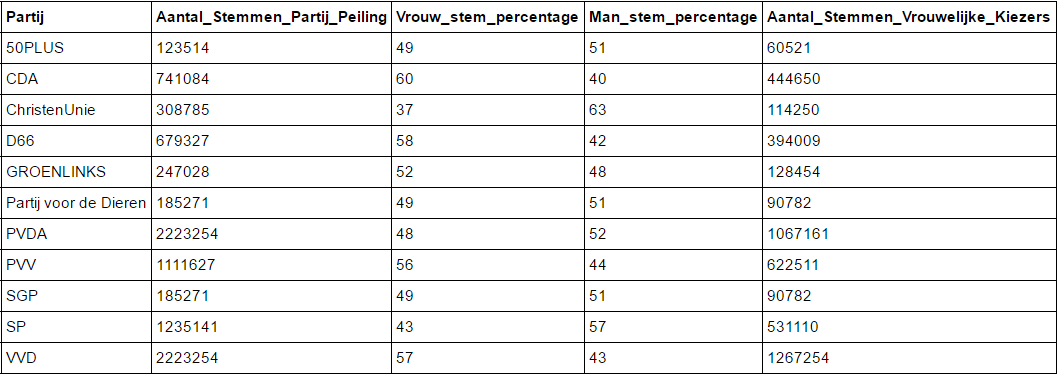
\includegraphics[width=\linewidth]	{stemmen_partij_df.png}
		\begin{center}
			Figuur 1: Tabel met totaal aantal stemmen dat een partij zou ontvangen, de verdeling vrouwen- en mannenstemmen(in percentages) en het aantal te verwachten vrouwen stemmen volgens de peiling. 
		\end{center}
\end{center}
\end{figure}

\paragraph{Het opstellen van de Tweede Kamer na uitvoering van de strategie.} 
Voor het uiteindelijk opstellen van de Tweede Kamer, wanneer alle vrouwelijke kiezers zich gecommitteerd hebben aan één van de hieronder beschreven strategi\"{e}n, moet je uiteindelijk kijken hoeveel zetels de partijen bij de einduitslag hebben behaald. Daarmee bepaal je de succes van de strategie. Naast het aantal behaalde zetels per partij moet er ook gekeken worden naar het aantal stemmen dat de afzonderlijke kandidaten hebben ontvangen bij de einduitslag zoals deze was in 2012. Daarbij moet het aantal stemmen dat een mannelijke kandidaat kreeg worden vergelijken met het aantal stemmen dat een vrouwelijke kandidaat zou hebben gekregen wanneer alle vrouwelijk kiezers zich hadden gecommitteerd aan één van de strategi\"{e}n. Het opstellen van de Tweede Kamer na uitvoering van één van de strategi\"{e}n werkt hetzelfde voor elke van de hieronder uiteengezette strategi\"{e}n, wat betreft de bevolkingsgroep vrouwen in Nederland, en gaat als volgt: 
\begin{itemize}
	\item
Als eerst wordt er gekeken hoeveel zetels een partij heeft ontvangen bij de uitslag van de Tweede Kamerverkiezingen van 2012. 
	\item
Vervolgens wordt, na toewijzing van de stemmen van vrouwelijke kiezers op vrouwelijke kandidaten, geteld hoeveel kandidaten(mannelijke én vrouwelijke kandidaten) er boven de kiesdrempel komen. Daarbij moet genoteerd worden dat na uitvoering van de strategie de mannelijke kandidaten evenveel stemmen hebben ontvangen als wanneer de strategie niet wordt uitgevoerd. De reden hiervoor is dat het theoretisch mogelijk is dat de mannelijke kandidaten  enkel stemmen hebben ontvangen van mannelijke kiezers. Ook al is dit onwaarschijnlijk, kunnen we dit niet weten en zullen we ook geen stemmen van de mannelijke kandidaten aftrekken en is het aantal stemmen dat een mannelijke kandidaat ontvangt hetzelfde als bij de verkiezingsuitslag van 2012.
	\item
Nadat we, na uitvoering van een strategie, hebben geteld hoeveel kandidaten genoeg stemmen hebben ontvangen om boven de voorkeursdrempel uit te komen kijken we per partij of de partij meer zetels heeft ontvangen dan dat er kandidaten voor die partij boven de voorkeursdrempel zijn gekomen. 
	\item
Als de partij meer zetels heeft ontvangen dan er voor de partij kandidaten boven de voorkeursdrempel zijn gekomen, worden de resterende zetels vergeven aan de hoogst genoteerde kandidaten op de kandidatenlijst van de partij(mits deze kandidaten dus niet genoeg stemmen hebben ontvangen om boven de voorkeursdrempel uit te komen).
\end{itemize}


\subsubsection*{Strategie 1: Vrouwelijke kiezers stemmen op top N vrouwelijke kandidaten.}

\paragraph{Aannames.}
\begin{itemize}
	\item
Alle stemgerechtigde vrouwen waarvan de peiling aangeeft dat zij gaan stemmen doen in theorie mee aan de strategie.
	\item
Vrouwelijke kiezers stemmen daarbij op de top \textit{N} vrouwelijke kandidaten van de partij waar zij toch al op wilden stemmen.
\end{itemize}

\paragraph{Regels.}
\begin{itemize}
	\item
Het aantal vrouwelijke stemmen die een partij volgens de peiling zou gaan krijgen, worden willekeurig verdeeld over de top \textit{N} vrouwelijke kandidaten die op de kandidatenlijst van de partij staan, waarbij \textit{N} staat voor het maximaal aantal vrouwen per partij dat volgens de peiling in de Tweede Kamer gestemd had kunnen worden.
 	\item
Elke partij krijgt een eigen \textit{N}:
	\begin{itemize}
		\item
In het geval de partij minder vrouwen op de kandidatenlijst had staan dan dat de partij, volgens de peiling, aan zetels zou gaan ontvangen is \textit{N} gelijk aan het totaal aantal vrouwen op de kandidatenlijst van de partij.
		\item
In het geval de partij meer vrouwelijke kandidaten op de kandidatenlijst had staan dan dat de partij, volgens de peiling, aan zetels zou gaan ontvangen is \textit{N} gelijk aan het totaal aantal zetels die de partij volgens de peiling zou gaan ontvangen.
\end{itemize} 	
\end{itemize}

\paragraph{Verdelingen zetels en aantal vrouwelijke kandidaten.}
Zoals hierboven al vermeld wordt per partij de top \textit{N} vrouwelijke kandidaten bepaald door het totaal aantal zetels dat een partij zou gaan ontvangen volgens de peiling, mits de partij minstens een even groot aantal vrouwelijke kandidaten op de kandidatenlijst had staan als dat de partij aan aantal zetels zou gaan ontvangen. Wanneer het aantal vrouwelijke kandidaten op de kandidatenlijst van de partij minder is dan het aantal zetels dat de partij  zou gaan ontvangen volgens de peiling, is de top \textit{N} voor de partij gelijk aan het totaal aantal vrouwelijke kandidaten op de kandidatenlijst van de partij. 
In de grafiek hieronder is te zien hoe de verdeling is. Alle partijen links van de stippellijn hadden meer vrouwelijke kandidaten op de kandidatenlijst staan dan dat zij zetels zouden gaan ontvangen volgens de peiling. Alle partijen rechts van de stippellijn hadden minder vrouwelijke kandidaten op de kandidatenlijst staan dan dat zij zetels gaan ontvangen.
 
\begin{figure}[H]
\begin{center}
	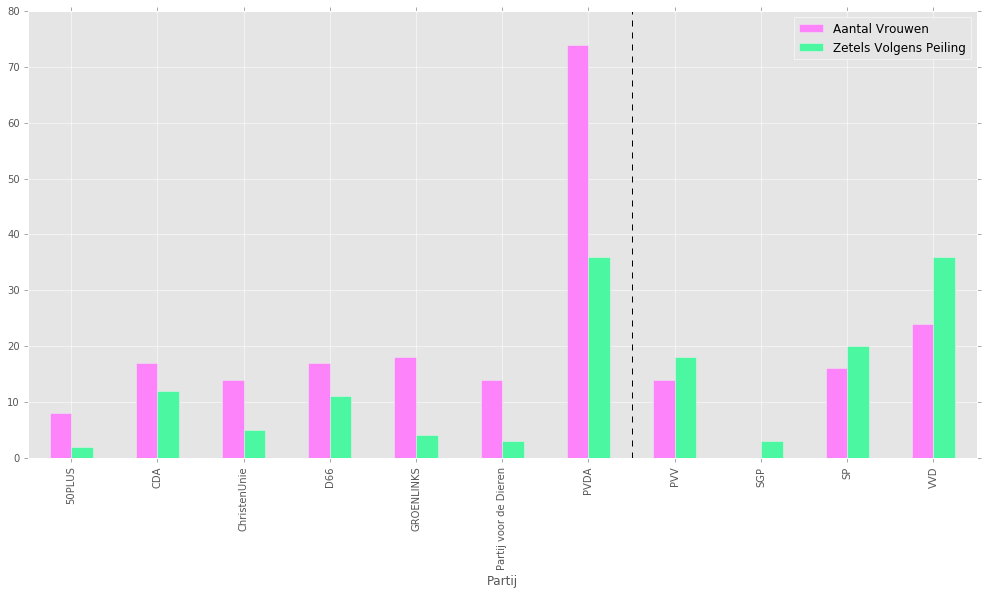
\includegraphics[width=\linewidth]	{Aantal_vrouwen_aantal_zetels.png}
		\begin{center}
			Figuur 2: Het aantal vrouwen op de kandidatenlijst(paars) en het aantal zetels volgens de peilingen(groen) per partij.
		\end{center}
\end{center}
\end{figure}

\paragraph{Maximaal aantal vrouwen per partij(top \textit{N}) dat in de Tweede Kamer gekozen kan worden.}
In Figuur 2 is te zien hoeveel zetels een partij zou gaan ontvangen volgens de peiling en hoeveel vrouwelijke kandidaten de partij op de kandidatenlijst had staan. In Figuur 3 hieronder is daaruit voortvloeiend te zien hoeveel vrouwelijke kandidaten er per partij maximaal in de Tweede Kamer gekozen hadden kunnen worden. In de grafiek is dus per partij het aantal (\textit{N}) vrouwelijke kandidaten te zien waarover de stemmen van de vrouwelijke kiezers op de partij verdeeld zullen worden.  
\\
Vanwege het feit dat de SGP helemaal geen vrouwelijke kandidaten op de kandidatenlijst heeft staan en de PVV, de SP en de VVD volgens de peiling meer zetels zullen gaan ontvangen dan dat zij vrouwelijke kandidaten op de kandidatenlijsten hebben staan komt het totaal aantal vrouwelijke kandidaten dat volgens de peiling in de Tweede Kamer gekozen kan worden uit op 127. 
\todo{beschrijf waar die 23 mannen dan vandaan komen.}

\begin{figure}[H]
\begin{center}
	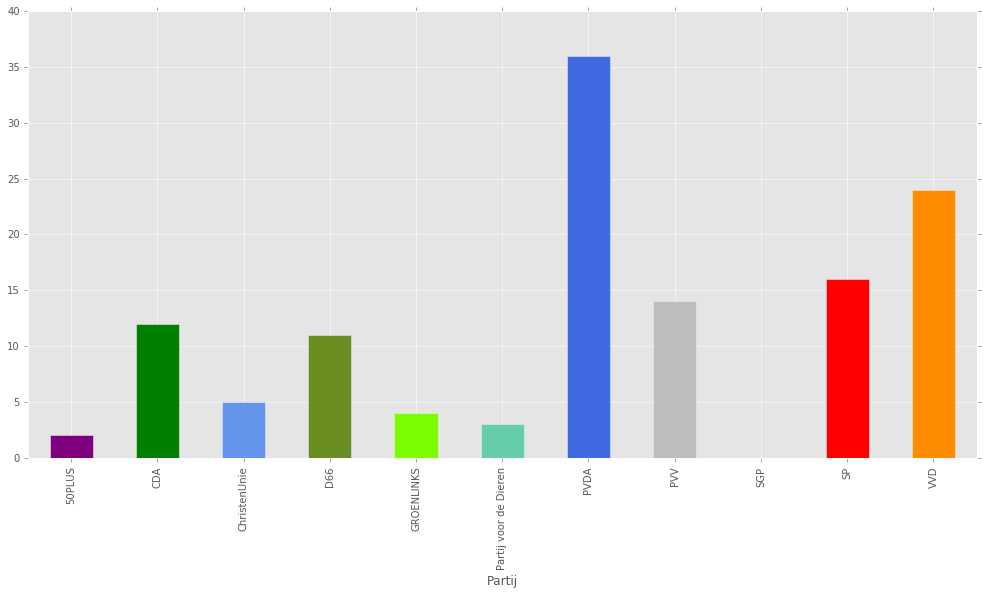
\includegraphics[width=\linewidth]	{aantal_vrouwen_per_partij_in_tweede_kamer_volgens_peiling.png}
		\begin{center}
			Figuur 3: Het aantal vrouwen op de kandidatenlijst per partij dat in de Tweede Kamer gekozen kan worden(de kleuren de staven zijn in de kleuren van de partijen). De waarden staan voor de top \textit{N} vrouwelijke kandidaten per partij.   
		\end{center}
\end{center}
\end{figure}

\paragraph{Het toewijzen van de stemmen aan de vrouwelijke kandidaten.}
Zoals te zien in Figuur 1, hebben we berekend hoeveel stemmen een partij, volgens de peiling, zou gaan ontvangen en hoeveel stemmen van vrouwelijke kiezers een partij zou gaan ontvangen. Nu gaan we de vrouwelijke stemmen toewijzen aan vrouwelijke kandidaten op de kandidatenlijsten. Ter illustratie nemen we weer de PVDA als voorbeeld. De PVDA zou,volgens de peiling en zoals in de vorige paragraaf berekend, een totaal van 1.067.161 stemmen gaan ontvangen. Deze stemmen worden verdeeld over de top \textit{N} vrouwelijke kandidaten van de PVDA. Zoals eerder al vastgesteld, en te zien in Figuur 2, heeft de PVDA een \textit{N} = 36. De stemmen van vrouwelijke kiezers op de PVDA worden willekeurig(gelijk) verdeeld over de eerste 36 vrouwelijke kandidaten op de kandidatenlijst van de PVDA. Daarmee krijgen de top 36 vrouwelijke kandidaten van de PVDA (ongeveer) het aantal van (1.067.161/36 = ) 29.643 stemmen per vrouwelijke kandidaat. Dat is ruim boven de voorkeursdrempel van 15.708 stemmen. In de grafiek in Figuur 4 hieronder is te zien dat, met deze strategie, alle top \textit{N} vrouwelijke kandidaten van alle partijen(behalve het vrouwloze SGP) boven de voorkeursdrempel van 15.708 stemmen komen. De stippellijn in de grafiek geeft de voorkeursdrempelwaarde aan. 

  
\begin{figure}[H]
\begin{center}
	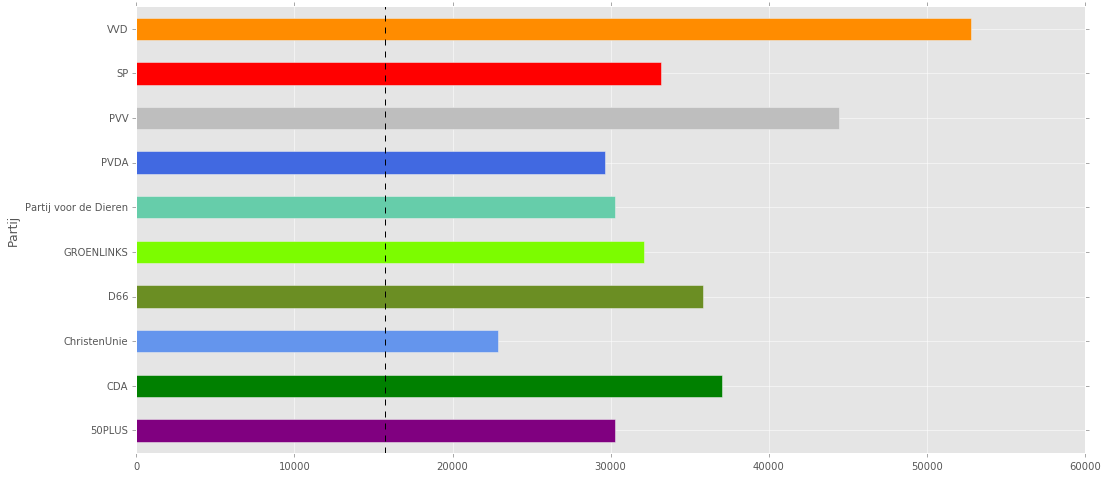
\includegraphics[width=\linewidth]	{stemmen_op_vrouwen_topN.png}
		\begin{center}
			Figuur 4: Grafiek met per partij de verdeling van de stemmen van vrouwelijk kiezers op de top \textit{N} vrouwelijke kandidaten. De SGP wordt niet in de grafiek getoond omdat deze partij geen vrouwelijke kandidaten op de kandidaten lijst heeft staan. 
		\end{center}
\end{center}
\end{figure}

Na het uitvoeren van de strategie 1 en het opstellen van de Tweede Kamer zoals eerder in dit hoofdstuk beschreven, levert strategie 1 een Tweede Kamer op waarin 122 vrouwen en 28 mannen plaatsnemen. Daarmee zijn vrouwen(met 81.33\%) ruim in hogere mate vertegenwoordigd dan mannen(met 18.67\%). In de cirkeldiagram(Figuur 5) hieronder is de verdeling goed te zien. 

\begin{figure}[H]
\begin{center}
	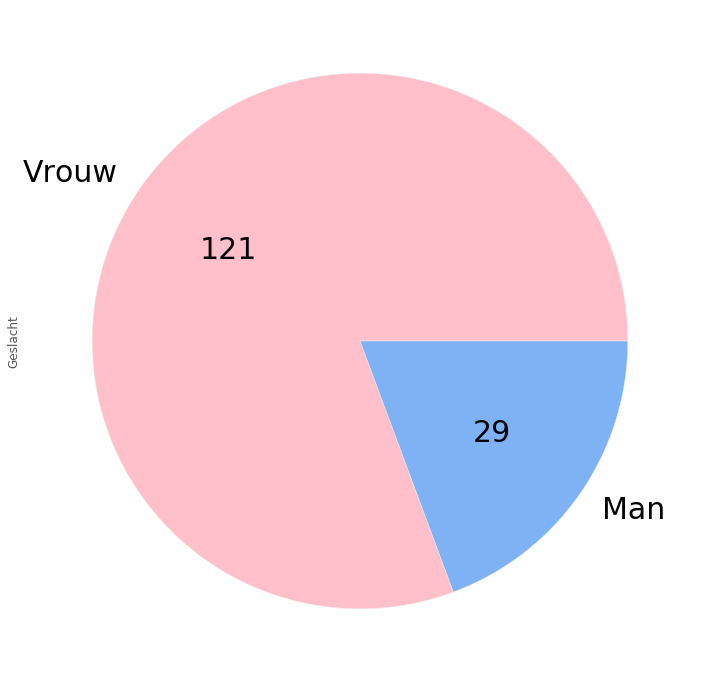
\includegraphics[width=0.7\linewidth]{pie_chart_topN.png}
		\begin{center}
			Figuur 5: Na uitvoering van de strategie nemen er 122 vrouwen(81.33\%) en 28 mannen(18.67\%) plaats in de Tweede Kamer. 
		\end{center}
\end{center}
\end{figure}

\newpage
\paragraph{Minder vrouwen dan 127 vrouwen in de Tweede Kamer na uitvoering van strategie 2.}
De reden dat er niet 127 vrouwen maar 'slechts' 122 vrouwen in de Tweede Kamer plaatsnemen na uitvoering van strategie 1 ligt ten grondslag aan een aantal factoren. Zo hadden het merendeel van de partijen die zetels ontvingen een mannelijke kandidaat als lijsttrekker en ontvingen deze lijsttrekkers de meeste stemmen in vergelijking met alle andere kandidaten van dezelfde partij. Hierdoor viel er uiteindelijk bij zowel de 50PLUS, de ChristenUnie als de SP één vrouwelijke kandidaat af. Daarnaast had de SP minder zetels behaald bij de einduitslag dan zij volgens de peiling zou gaan ontvangen. Hierdoor viel ook bij de SP nog een vrouwelijke kandidaat af. Ook de Partij voor de Dieren ontving minder zetels bij de einduitslag dan zij volgens de peiling zouden gaan ontvangen en, ondanks het feit dat zij een vrouwelijke lijsttrekker hadden in de persoon van Marianne Thieme, resulteerde dit in één afgevallen vrouwelijke kandidaat. Dit komt op een totaal van vijf afgevallen vrouwelijke kandidaten, oftewel een totaal van (127 - 5 = ) 122 vrouwen in de Tweede Kamer na uitvoering van strategie 1.  

\subsubsection*{Strategie 2: Vrouwelijke kiezers stemmen op een willekeurige vrouwelijke kandidaat.}

\paragraph{Aannames.}
\begin{itemize}
	\item
Alle stemgerechtigde vrouwen waarvan de peiling aangeeft dat zij gaan stemmen doen in theorie mee aan de strategie.
	\item
Vrouwen stemmen op een willekeurige vrouwelijke kandidaat van de partij waarop zij toch al wilden stemmen.
\end{itemize}

\paragraph{Regels.}
\begin{itemize}
	\item
Het aantal stemmen van vrouwelijke kiezers die een partij krijgt, worden willekeurig verdeeld over het alle vrouwelijke kandidaten die op de kandidatenlijst staan van de partij. 	 	
\end{itemize}

\paragraph{Het toewijzen van de stemmen aan de vrouwelijke kandidaten.}
Zoals te zien in Figuur 1, hebben we berekend hoeveel stemmen een partij, volgens de peiling, zou ontvangen en hoeveel stemmen van vrouwelijke kiezers een partij zou gaan ontvangen. Nu gaan we de vrouwelijke stemmen toewijzen aan vrouwelijke kandidaten op de kandidatenlijsten. Ter illustatie nemen we weer de PVDA als voorbeeld. De PVDA zou,volgens de peiling en zoals in de vorige paragraaf berekent, een totaal van 1.067.161 stemmen gaan ontvangen. Deze stemmen worden willekeurig verdeeld over alle vrouwelijke kandidaten op de kandidatenlijst van de PVDA. De PVDA heeft totaal het aantal van 74 vrouwelijke kandidaten op de kandidatenlijst staan. Daarmee krijgen de 74 vrouwelijke kandidaten van de PVDA (ongeveer) het aantal van (1.067.161/74 = ) 14.421 stemmen per vrouwelijke kandidaat. Dat is net onder de voorkeursdrempel van 15.708 stemmen. In de grafiek in Figuur 6 hieronder is te zien dat, met deze strategie, van welke partij de vrouwelijke kandidaten boven de voorkeursdrempel komen en welke eronder. De stippellijn geeft de voorkeursdrempel aan. Bij de partijen die rechts van de stippellijn uitkomen hebben alle vrouwelijke kandidaten meer stemmen dan de voorkeursdrempel. Bij de partijen die links van de stippellijn uitkomen hebben alle vrouwelijke kandidaten minder stemmen dat de voorkeursdrempel.  

\begin{figure}[H]
\begin{center}
	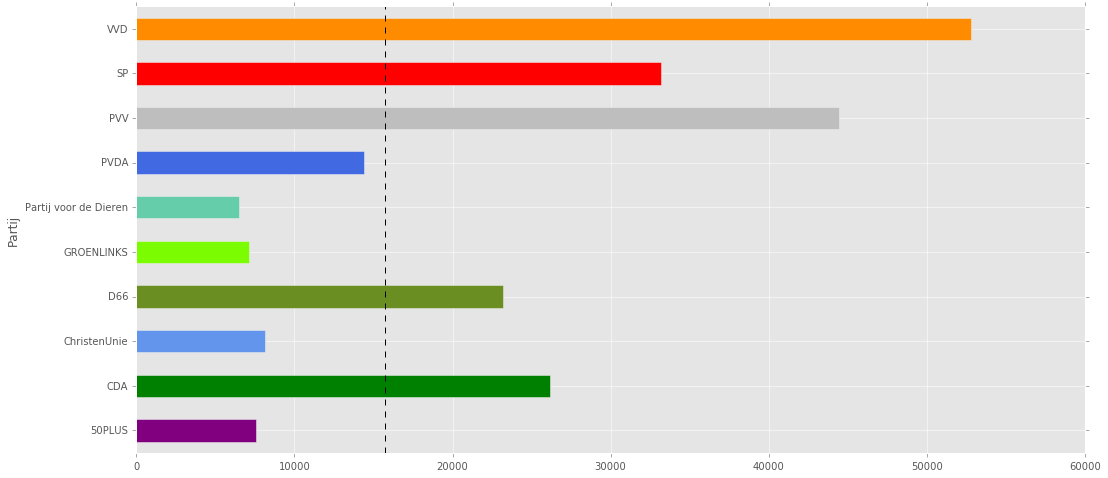
\includegraphics[width=\linewidth]	{stemmen_op_vrouwen_willekeurig.png}
		\begin{center}
			Figuur 6: Grafiek met per partij de verdeling van de stemmen van vrouwelijk kiezers op alle vrouwelijke kandidaten van de partij. De SGP wordt niet in de grafiek getoond omdat deze partij geen vrouwelijke kandidaten op de kandidaten lijst heeft staan. 
		\end{center}
\end{center}
\end{figure}

Na het uitvoeren van de strategie 1 en het opstellen van de Tweede Kamer zoals eerder in dit hoofdstuk beschreven, levert strategie 2 uiteindelijk een Tweede Kamer op waarin 99 vrouwen en 51 mannen plaatsnemen. Daarmee zijn vrouwen(met 66\%) ruim in hogere mate vertegenwoordigd dan mannen(met 34\%) maar is er net geen tweederde meerderheid die nodig is om een grondwetswijziging op gang te zetten. In de cirkeldiagram(Figuur 7) hieronder is de verdeling goed te zien. 

\begin{figure}[H]
\begin{center}
	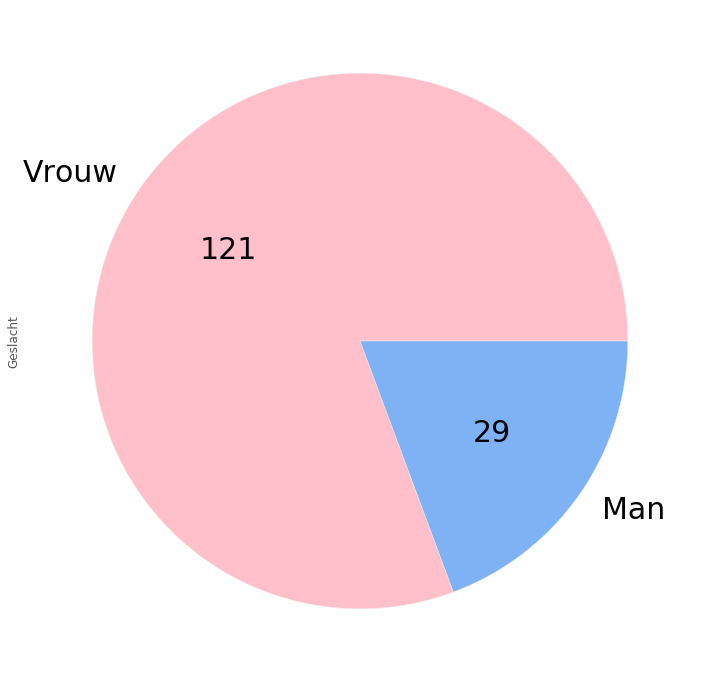
\includegraphics[width=0.7\linewidth]{pie_chart_topN.png}
		\begin{center}
			Figuur 7: Na uitvoering van de strategie nemen er 99 vrouwen(66\%) en 51 mannen(34\%) plaats in de Tweede Kamer. 
		\end{center}
\end{center}
\end{figure}

\paragraph{Minder vrouwen in de Tweede Kamer d.m.v. uitvoering van strategie 2 dan d.m.v. uitvoering van strategie 1.}
De reden dat er, na uitvoering van strategie 2, 99 vrouwen in de Tweede Kamer plaatsnemen en dat 23 vrouwen minder zijn dan bij strategie 1 ligt ten grondslag aan aan tweetal factoren. Ten eerste, door uitvoering van strategie 2, krijgen de vrouwelijke kandidaten van de PVDA, GROENLINKS, de ChristenUnie en 50PLUS minder stemmen dan de voorkeursdrempel. Hierdoor vallen bij de PVDA 17 vrouwelijke kandidaten af, bij GROENLINKS alsmede de ChristenUnie vallen er 2 vrouwelijke kandidaten af. Bij 50PLUS valt er 1 vrouwelijke kandidaat af. Ten tweede, heeft het CDA in de persoon van Pieter Omtzigt een kandidaat die met 36.750 stemmen meer stemmen heeft ontvangen dan de vrouwelijke kandidaten van het CDA hebben ontvangen(en tevens heeft Pieter Omtzigt meer stemmen ontvangen dan de voorkeursdrempel). Daarom valt ook bij het CDA 1 vrouwelijke kandidaat af in vergelijking met uitvoering van strategie 2. Geen enkele partij krijgt meer vrouwen in de Tweede Kamer na uitvoering van strategie 2 ten opzichte van strategie 1.   

\subsubsection*{Strategie 3: Vrouwelijke kiezers stemmen willekeurige op één van de eerste 15 vrouwelijke kandidaten van een partij.}

\paragraph{Aannames.}
\begin{itemize}
	\item
Alle stemgerechtigde vrouwen waarvan de peiling aangeeft dat zij gaan stemmen doen in theorie mee aan de strategie.
	\item
Vrouwelijke kiezers stemmen op de top 15 of top \textit{N} vrouwelijke kandidaten van de partij waar zij toch al op wilden stemmen.
\end{itemize}

\paragraph{Regels.}
\begin{itemize}
\item
Elke partij krijgt een eigen \textit{N}:
	\begin{itemize}
		\item
Wanneer een partij 15 of meer vrouwelijke kandidaten op de kandidatenlijst heeft staan geldt voor de partij 	\textit{N} = 15.
		\item
Wanneer een partij minder dan 15 vrouwelijke kandidaten op de kandidatenlijst heeft staan geldt voor de partij \textit{N} = het totaal aantal vrouwelijke kandidaten wat de partij op de kandidatenlijst heeft staan. 	
	\end{itemize}
\end{itemize}

\paragraph{Partijen met minstens 15 vrouwelijke kandidaten op de kandidatenlijst en partijen met minder dan 15(\textit{N}) vrouwelijke kandidaten op de kandidatenlijst.}
Hieronder is in de grafiek te zien welke partijen er voldoen aan de drempel van 15 vrouwelijke kandidaten op de kandidatenlijst om de stemmen die de partij van de vrouwelijke kiezers, volgens de peiling, zou gaan ontvangen te verdelen over de top 15 vrouwelijke kandidaten. We zien dat bij D66, GROENLINKS, de PVDA, het CDA, de SP en de VVD de stemmen van vrouwelijke kiezers over de top 15 vrouwelijke kandidaten verdeeld kunnen worden. Bij de Partij voor de Dieren, de ChristenUnie, 50PLUS en de PVV moeten de stemmen van vrouwelijke kiezers die de partij, volgens de peiling, zou gaan ontvangen verdeeld worden over alle vrouwelijke kandidaten die deze partij op de kandidatenlijst heeft staan. Voor de Partij voor de Dieren, voor de ChristenUnie en voor de PVV geldt \textit{N} = 14. Voor de 50PLUS geldt \textit{N} = 8 en voor de SGP geldt \textit{N} = 0. 

\begin{figure}[H]
\begin{center}
	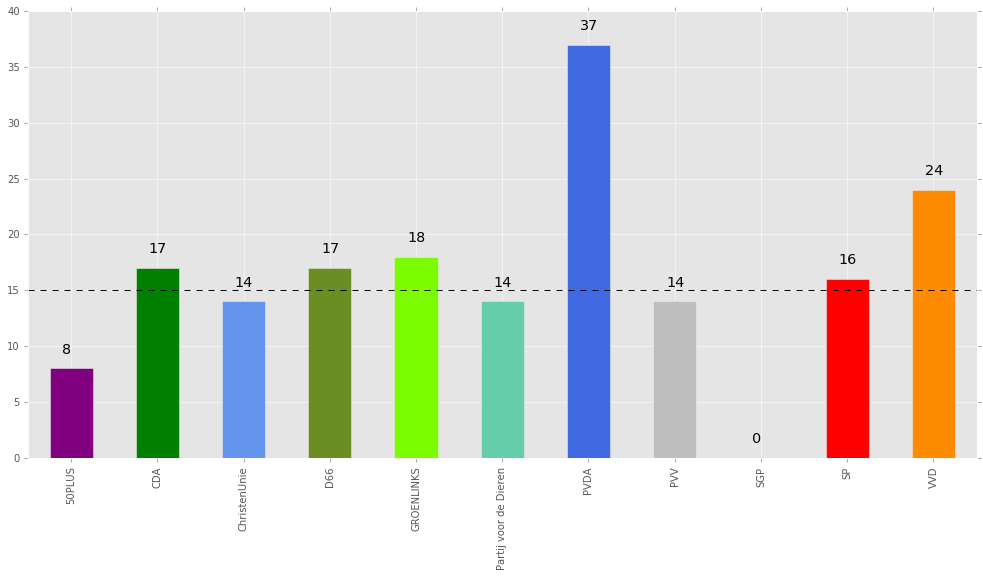
\includegraphics[width=\linewidth]	{top15_of_topN_kandidaten.png}
		\begin{center}
			Figuur 8: De grafiek toont bij welke partijen de vrouwelijke kiezers op de top 15 vrouwelijke kandidaten van de partij moeten gaan stemmen en van welke partijen de vrouwelijke kiezers op de het totaal aantal \textit{N} vrouwelijke kandidaten moeten gaan stemmen.   
		\end{center}
\end{center}
\end{figure}

\paragraph{Het toewijzen van de stemmen aan de vrouwelijke kandidaten.}
Zoals te zien in Figuur 1, hebben we berekend hoeveel stemmen een partij, volgens de peiling, zou ontvangen en hoeveel stemmen van vrouwelijke kiezers zullen een partij zou gaan ontvangen. Nu gaan we de vrouwelijke stemmen toewijzen aan vrouwelijke kandidaten op de kandidatenlijsten. Ter illustatie nemen we de PVDA en later de PVV als voorbeelden. Te beginnen met de PVDA. De PVDA zou,volgens de peiling en zoals eerder berekend, een totaal van 1.067.161 vrouwelijke stemmen gaan ontvangen. Deze stemmen worden willekeurig verdeeld over de top 15 vrouwelijke kandidaten van de PVDA. Dit wordt zo gedaan omdat de PVDA minstens 15 vrouwelijke kandidaten op de kandidatenlijst had staan. Daarmee krijgen de top 15 vrouwelijke kandidaten op de kandidatenlijst van de PVDA (ongeveer) het aantal van (1.067.161/15 = ) 71.144 stemmen per vrouwelijke kandidaat. Dat is ruim boven de voorkeursdrempel van 15.708 stemmen. Het volgende voorbeeld is de PVV. De PVV zal, volgens de peiling en zoals eerder berekent, een totaal van 622.511 vrouwelijke stemmen ontvangen. Het totaal aantal vrouwelijke kandidaten op de kandidatenlijst van de PVV is, in de vorige paragraaf, vastgesteld op 14. Daarmee krijgen de 14 vrouwelijke kandidaten op de kandidatenlijst van de PVV (ongeveer) het aantal van (622.511/14 = ) 44.465 stemmen per vrouwelijke kandidaat. Ook in dit voorbeeld is dat ruim boven de voorkeursdrempel van 15.708 stemmen. In de grafiek in Figuur 9 hieronder is te zien, door uitvoering van strategie 3, van welke partijen de top 15 vrouwelijke kandidaten of het \textit{N} aantal vrouwelijke kandidaten boven de voorkeursdrempel komen en welke eronder. De stippellijn geeft de voorkeursdrempel aan. Bij de partijen die rechts van de stippellijn uitkomen hebben alle vrouwelijke kandidaten meer stemmen dan de voorkeursdrempel. Bij de partijen die links van de stippellijn uitkomen hebben alle vrouwelijke kandidaten minder stemmen dat de voorkeursdrempel. 

\begin{figure}[H]
\begin{center}
	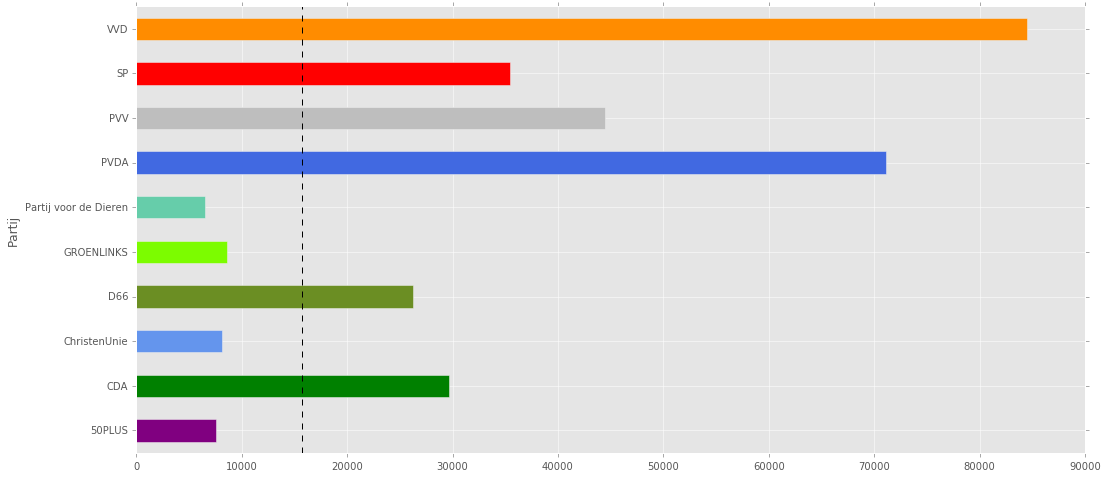
\includegraphics[width=\linewidth]	{stemmen_op_vrouwen_top15_of_topN.png}
		\begin{center}
			Figuur 9: Grafiek met per partij de verdeling van de stemmen van vrouwelijk kiezers op de top 15 of het \textit{N} aantal vrouwelijke kandidaten. De SGP wordt niet in de grafiek getoond omdat deze partij geen vrouwelijke kandidaten op de kandidaten lijst heeft staan. 
		\end{center}
\end{center}
\end{figure}

Na het uitvoeren van de strategie 1 en het opstellen van de Tweede Kamer zoals eerder in dit hoofdstuk beschreven, levert strategie 2 uiteindelijk een Tweede Kamer op waarin waarin 91 vrouwen  en 59 mannen plaatsnemen. Daarmee zijn vrouwen(met 60.67\%) in hogere mate vertegenwoordigd dan mannen(met 39.33\%). In de cirkeldiagram(Figuur 10) hieronder is de verdeling goed te zien. 

\begin{figure}[H]
\begin{center}
	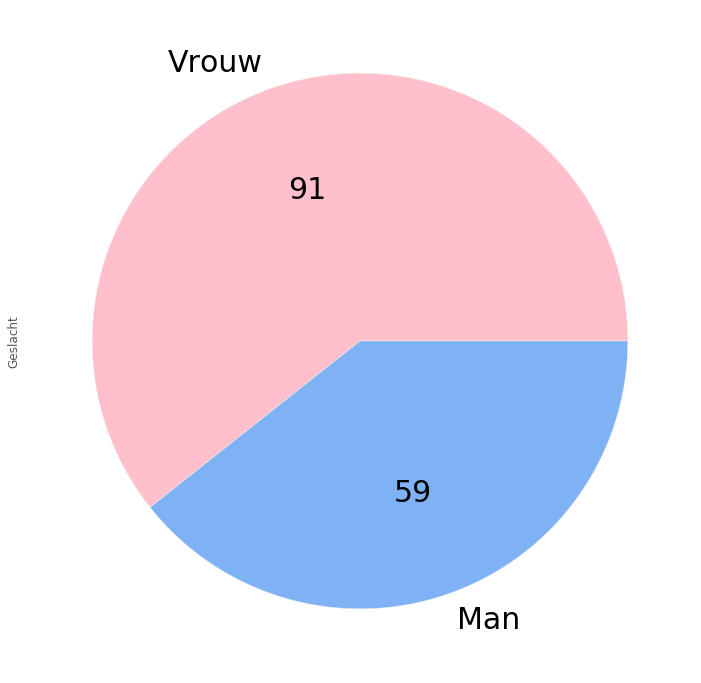
\includegraphics[width=0.7\linewidth]{pie_chart_top15_of_topN.png}
		\begin{center}
			Figuur 10: Na uitvoering van de strategie nemen er 91 vrouwen(60.67\%) en 59 mannen(39.33\%) plaats in de Tweede Kamer. 
		\end{center}
\end{center}
\end{figure}

\paragraph{Minder vrouwen in de Tweede Kamer d.m.v. uitvoering van strategie 3 dan d.m.v. uitvoering van strategie 2.}
De reden dat er, na uitvoering van strategie 3, 91 vrouwen in de Tweede Kamer plaatsnemen en dat er daarmee 8 vrouwen minder plaatsnemen in de Tweede Kamer dan bij strategie 2 het geval zou zijn ligt ten grondslag aan het feit dat er bij de VVD 8 vrouwelijke kandidaten afvallen ten opzichte van strategie 2. Dit komt omdat de stemmen niet verdeeld worden over alle 24 vrouwelijke kandidaten van de VVD maar over de top 15 vrouwelijke kandidaten van de VVD. De top 15 vrouwelijke kandidaten van de VVD ontvangen daardoor allen een zetel in de Tweede Kamer. Daarnaast ontvangt ook een 16e vrouwelijke kandidaat, in de persoon van Ingrid de Caluwé, een zetel in de Tweede Kamer vanwege haar plaats op de kandidatenlijst. Echter vallen de er 8 vrouwelijke kandidaten buiten de boot na uitvoering van strategie 3 ten opzichte van uitvoering van strategie 2. Daarmee komt het totale aantal vrouwen in de Tweede Kamer uit op (99 - 9 + 1 = ) 91.

\newpage
\section{Factoren & Invloed}
\label{sec:conc}

Hierin beantwoord je jouw hoofdvraag op basis van het eerder vergaarde bewijs.



\subsection{Acknowledgements}
Hier kan je bedanken wie je maar wilt.

\newpage
\section{Appendix}

% your refs

\bibliographystyle{plain}
\bibliography{MyThesis}

\appendix

%\input{appendix}


section{Slides}

% Example

\includepdf[nup=2x3 , pages=-]{sargent-lecture_slides.pdf}
 
\end{document}
